\documentclass[13pt]{article}

\usepackage{amsmath}
\usepackage{mathtools}
\usepackage[utf8]{inputenc}
\usepackage[english,greek]{babel}
\usepackage{graphicx}
\graphicspath{{media/}}
\usepackage[
  a4paper,
  top=2.5cm,
  bottom=2.5cm,
  left=2.5cm,
  right=2.5cm
]{geometry}
\usepackage{siunitx}
\usepackage{xcolor}
\usepackage{pdfpages}
\usepackage{soul}
\usepackage{listings}
\usepackage{subcaption}
\usepackage{caption}
\usepackage{biblatex}
\addbibresource{references.bib}

\newcommand{\eng}[1]{\foreignlanguage{english}{#1}}
\newcommand{\langeng}{\selectlanguage{english}}
\newcommand{\langgrc}{\selectlanguage{greek}}

\title{Βάσεις Δεδομένων\\[1.2ex]
        \Large ΥΠΌΤΙΤΛΟΣ}
\date{\today}
\author{Ίωνας Τσακίρης 03123077\footnote{\eng{el23077@mail.ntua.gr}}}


% Definition of \maketitle
\makeatletter         
\def\@maketitle{
\raggedright
\mbox{}\hfill
\begin{minipage}{2cm}
    
\includegraphics[width = 20mm,valign=b]{pyrforos}
\end{minipage}
\hfill
\begin{minipage}{12cm}
    {\Large \bfseries Εθνικό Μετσόβιο Πολυτεχνείο}\\ 
    {\Large Σχολή Ηλεκτρολόγων Μηχανικών και Μηχανικών\\Υπολογιστών}
\end{minipage}

\\[16ex]
\begin{center}
{\Huge \bfseries \@title }\\[4ex] 
{\Large  \@author}\\[4ex] 
\@date\\[8ex]
\end{center}}
\makeatother

\begin{document}
\pagenumbering{gobble}
\maketitle
\newpage
\tableofcontents
\newpage
\pagenumbering{arabic}

\section{\eng{Relational Diagram}}

\begin{figure}[h]
    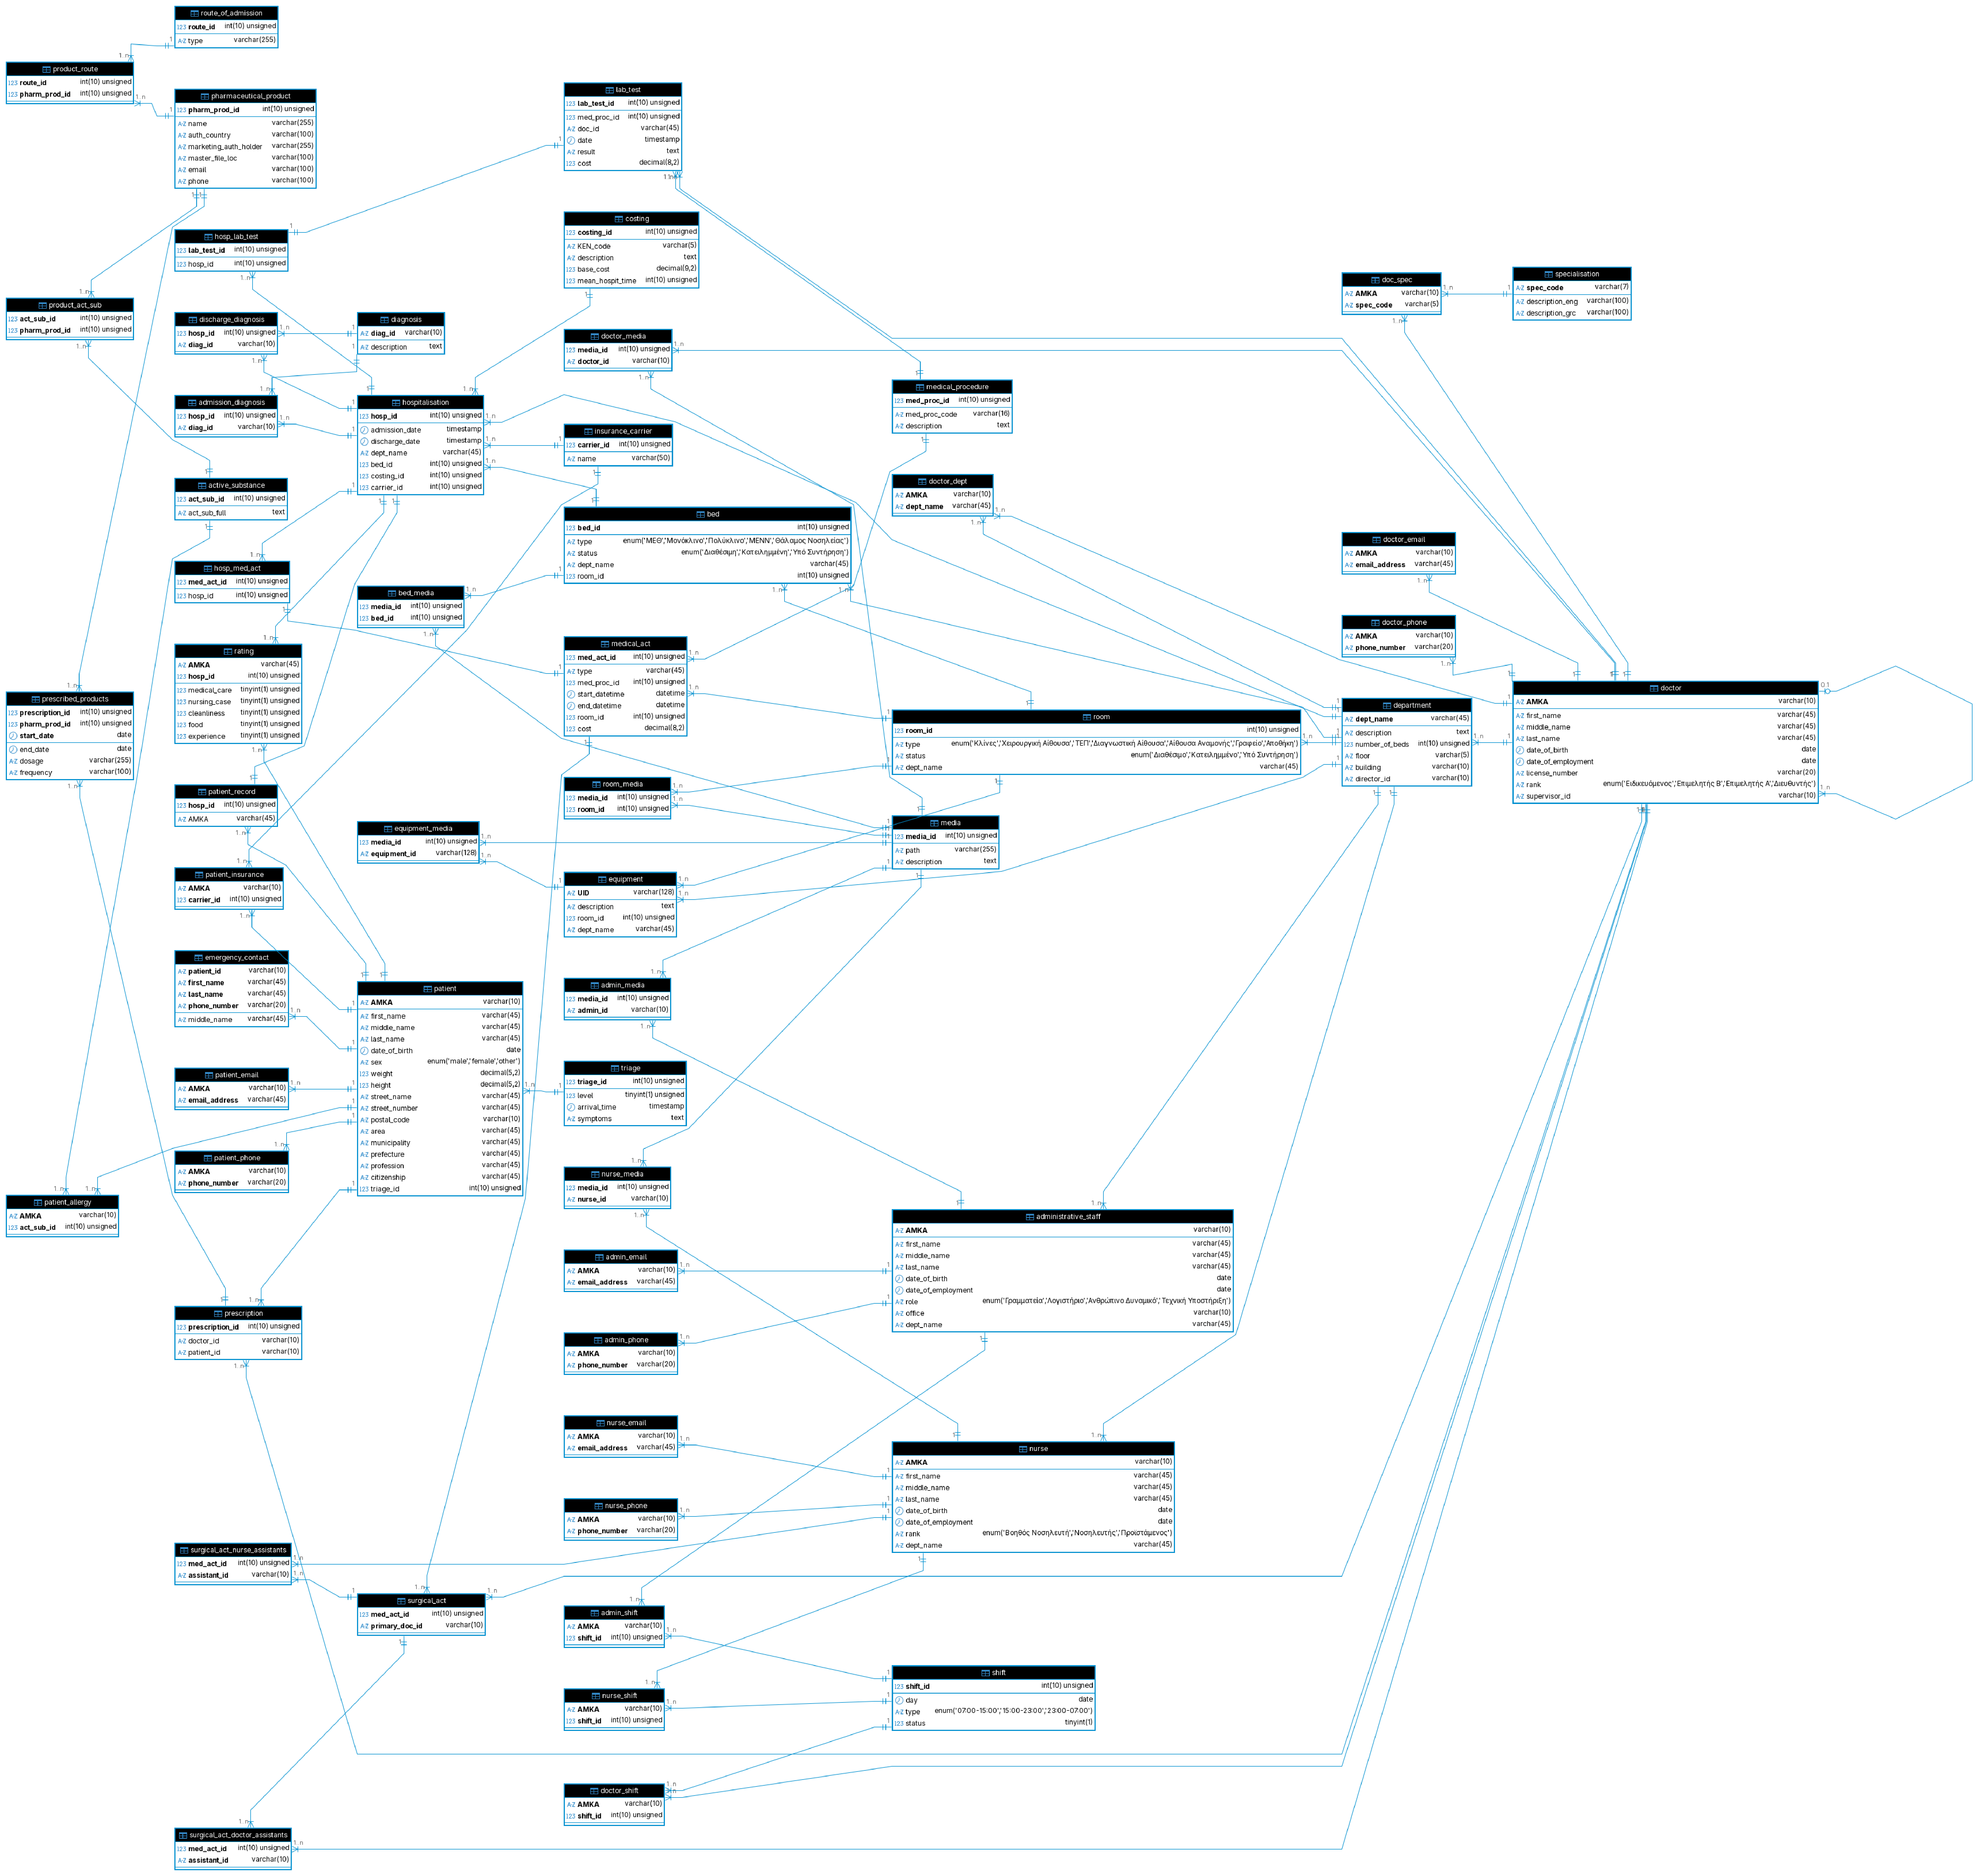
\includegraphics[width=0.9\linewidth]{../diagrams/relational.pdf}
    \caption{Σχεσιακό διάγραμμα βάσης}
    \label{fig:rel}
\end{figure}

\clearpage 

\section{\eng{ERD}}

\begin{figure}[h]
    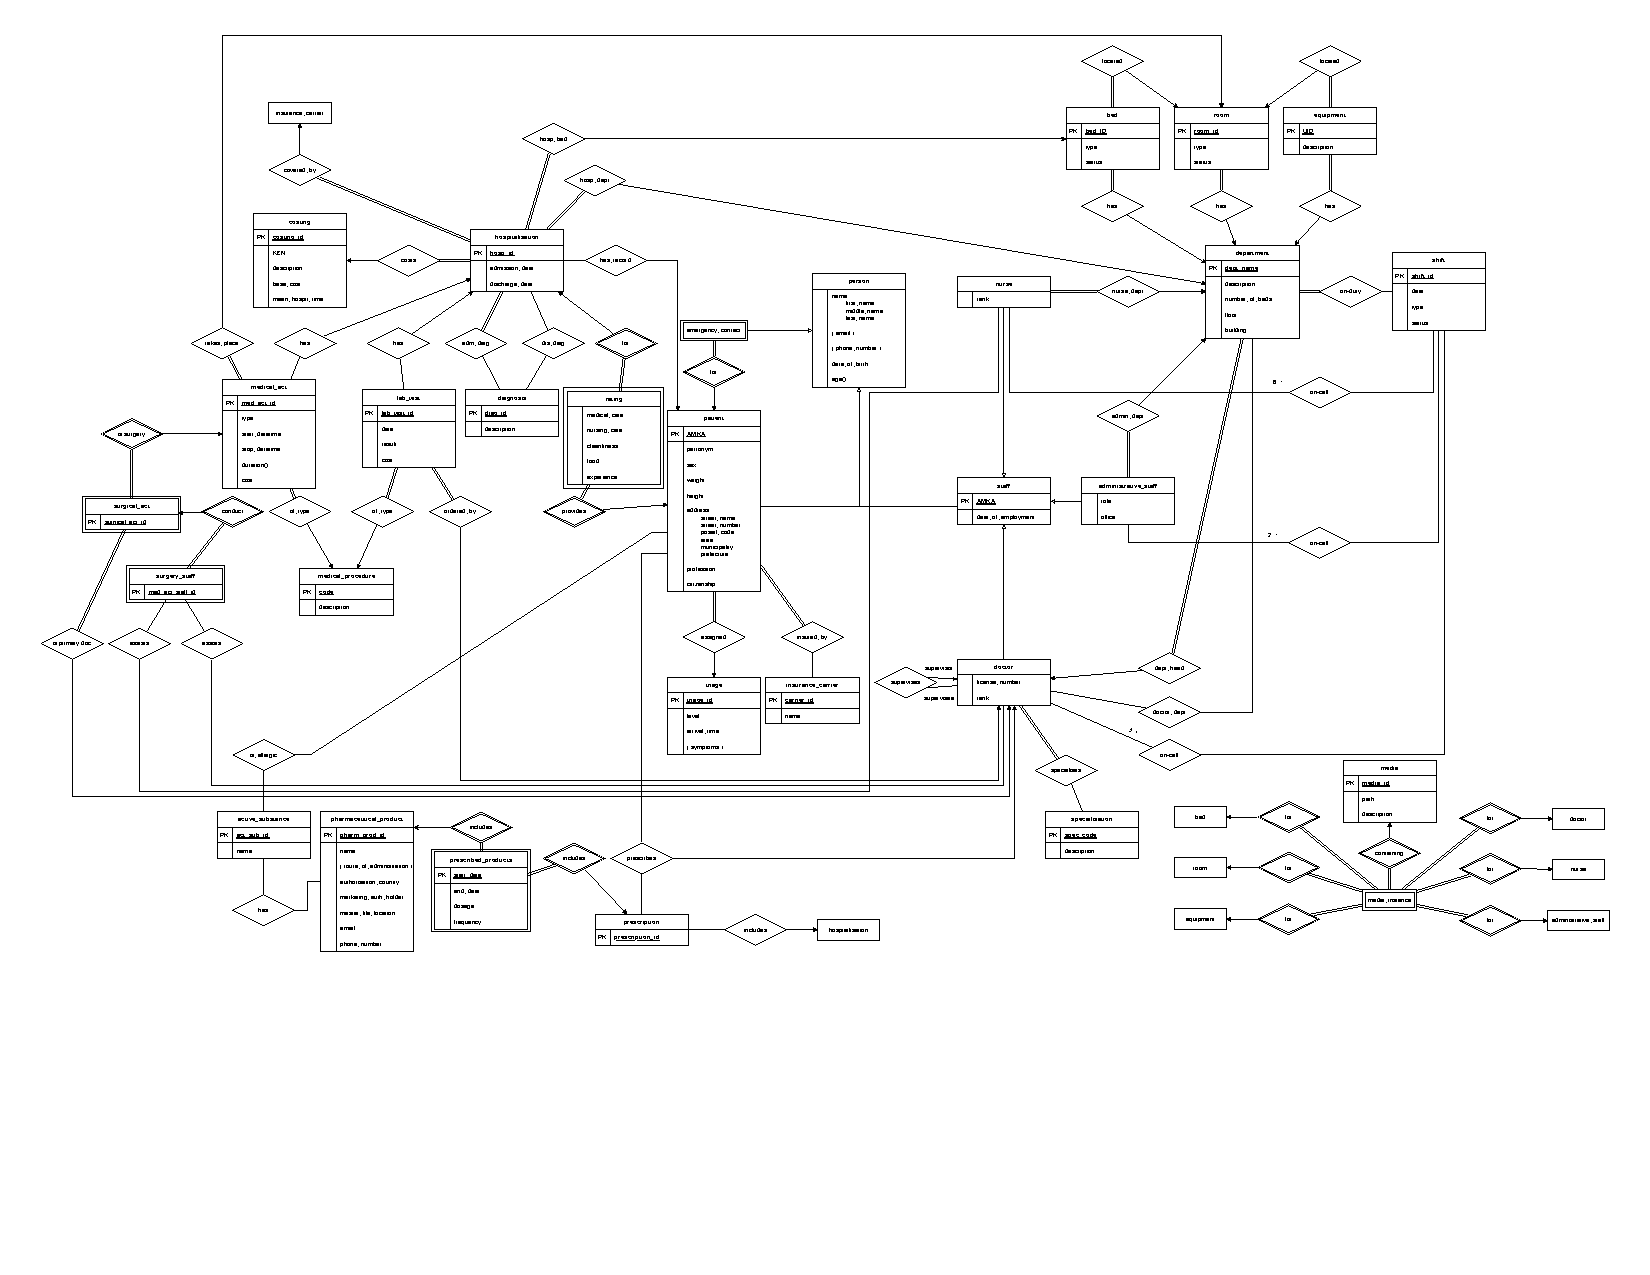
\includegraphics[width=\linewidth]{../diagrams/er.pdf}
    \caption{Διάγραμμα \eng{ER} βάσης}
    \label{fig:er}
\end{figure}

\subsection{\eng{Relations}}

\begin{itemize}
\tightlist
\item
  διοικητικό προσωπικό \textbf{είναι} προσωπικό
\item
  νοσηλευτής \textbf{είναι} προσωπικό
\item
  γιατρός \textbf{είναι} προσωπικό
\item
  επόπτης \textbf{είναι} γιατρός
\item
  γιατρός \textbf{μπορεί να έχει έναν} επόπτη
\item
    \textbf{απαγορεύεται η κυκλική αλυσίδα εποπτείας}
\item
  \textbf{κάθε} ειδικευόμενος \textbf{έχει έναν} επόπτη
\item
  διευθυντές \textbf{δεν έχουν} επόπτη
\item
  γιατρός \textbf{μπορεί να ανήκει σε \textgreater= 2} τμήματα
\item
    γιατρός \textbf{έχει \textgreater= 1} ειδικότητες

\item
  \textbf{κάθε} νοσηλευτής \textbf{έχει} βαθμίδα \textbf{και ανήκει σε
  ένα} τμήμα
\item
  \textbf{κάθε} τμήμα \textbf{έχει έναν} διευθυντή (γιατρό)
\item
  \textbf{κάθε} τμήμα \textbf{έχει} δωμάτια
\item
  \textbf{κάθε} τμήμα \textbf{έχει} κλίνες
\item
  \textbf{κάθε} κλίνη \textbf{βρίσκεται σε} δωμάτιο
\item
  \textbf{κάθε} ασθενής \textbf{έχει} ασφαλιστικό φορέα
\item
    \textbf{κάθε} ασθενής \textbf{έχει \textgreater=1} καταθέσεις διαλογής (στο ιστορικό
  του)
\item
  ασθενής \textbf{μπορεί να έχει \textgreater=1} νοσηλείες (στο ιστορικό
  του)
\item
  \textbf{κάθε} βάρδια \textbf{κάθε} τμήματος \textbf{έχει \textgreater=
  3} γιατρούς \textbf{και \textgreater=6} νοσηλευτές \textbf{και
  \textgreater= 2} διοικητικούς υπαλλήλους
\item
  \textbf{αν σε} βάρδια \textbf{υπάρχει} ειδικευόμενος γιατρός
  \textbf{τότε πρέπει να υπάρχει \textgreater= 1} γιατρός βαθμίδας
  Επιμελητής Α' \textbf{ή \textgreater= 1} διευθυντής
\item
  ασθενής \textbf{που χρειάζεται} νοσηλεία \textbf{εισάγεται σε} τμήμα
  \textbf{με} κλίνη
\item
    \textbf{κάθε} vοσηλεία \textbf{έχει} κοστολόγηση
\item
  νοσηλεία \textbf{μπορεί να συνδέεται με \textgreater= 1}
  εργαστηριακές\_εξετάσεις
\item
  νοσηλεία \textbf{μπορεί να συνδέεται με \textgreater= 1}
  ιατρικές\_πράξεις
\item
  νοσηλεία \textbf{μπορεί να συνδέεται με \textgreater= 1}
  ιατρικές\_επεμβάσεις
\item
  \textbf{κάθε} ιατρική\_επέμβαση \textbf{έχει} κύριο χειρούργο
  \textbf{και \textgreater= 0} βοηθούς (προσωπικό)
\item
    \textbf{κάθε} φαρμακευτική\_αγωγή \textbf{εκδίδεται από} γιατρό \textbf{για} ασθενή
\item
  (γιατρός, ασθενής, φάρμακο, ημερομηνίας έναρξης) \textbf{είναι
  \eng{superkey}}
\end{itemize}

\subsection{\eng{Constraints}}

\begin{itemize}
\tightlist
\item
  βαρδιες χωρίζονται σε πρωινές, απογευματινές και νυχτερινές
\item
  μέγιστο πλήθος βαρδιών:

  \begin{itemize}
  \tightlist
  \item
    γιατρός: 15
  \item
    νοσηλευτής: 20
  \item
    διοικητικό προσωπικό: 25
  \end{itemize}
\item
  προσωπικό δεν μπορεί να έχει διαδοχικές βάρδιες (πρωί \textbf{ΚΑΙ}
  απόγευμα \textbf{\emph{Ή}} απόγευμα \textbf{ΚΑΙ} νύχτα
  \textbf{\emph{Ή}} νύχτα \textbf{ΚΑΙ} πρωί (επόμενης) )
\item
  προσωπικό δεν μπορεί να έχει \textgreater=3 διαδοχικές νυστερινές
  βάρδιες
\item
    εξυπηρέτηση διαλογής βάσει επιπέδου επείγοντος με \eng{FIFO}
\item
  δύο επεμβάσεις δεν μπορούν να πραγματοποιούνται ταυτόχρονα στον ίδιο
  χώρο και με το ίδιο προσωπικό
\item
  ασθενείς μπορεί να έχουν καταγεγραμμένες αλλεργίες σε δραστικές ουσίες
\item
  απαγορεύεται η συνταγογράφηση φαρμάκων με δραστική ουσία στην οποία
  είναι αλλεργικός ο ασθενής
\end{itemize}

\subsection{Υποθέσεις και Σημειώσεις}
\begin{itemize}
    \item
Κάθε τμήμα διαθέτει αίθουσες με κάποιο τύπο (χειρουργικές, επεμβάσεων, κ.λπ), κατάσταση και μοναδική αρίθμηση.

    \item
Η διεύθυνση ασθενών εμπεριέχει τα στοιχεία του ΕΜΕπ

    \item
Χάριν απλότητας της υλοποίησης, θεωρούμε ότι κάθε κοστολόγηση μπορεί να συνδέεται με το πολύ έναν ασφαλιστικό φορέα. Στην περίπτωση, δηλαδή, παράλληλης ασφάλισης του ασθενούς, μόνο ένας φορέας καλύπτει κάθε κοστολόγηση.

    \item
Οι εικόνες αναπαρίστανται ως \eng{blobs}.

    \item
Επιταχύνουμε, στο \eng{install.sql}, την εισαγωγή δεδομένων βάσει του ερωτήματος \texttt{A.6}\footnote{\eng{https://dev.mysql.com/doc/workbench/en/workbench-faq.html#faq-workbench-increase-performance}}.

    \item
        Οι γιατρικές ειδικότητες προκύπτουν από τη λίστα του ΓεΣΥ \cite{gesy_spec}.

    \item
Στο δοθέν αρχείο ΕΛΛΗΝΙΚΗ\_ΟΝΟΜΑΤΟΛΟΓΙΑ\_ΚΑΙ\_ΚΩΔΙΚΟΠΟΙΗΣΗ\_ΤΩΝ\_ΙΑΤΡΙΚΩΝ\_ΠΡΑΞΕΩΝ, κάποιες τιμές είναι μη μοδανικές, και παραλείπονται απο τη βάση.
\langeng
\begin{lstlisting}
+---------+------+---------------------------------------------------+
| Level   | Code | Message                                           |
+---------+------+---------------------------------------------------+
| Warning | 1062 | Duplicate entry 'I212243' for key 'med_proc_code' |
| Warning | 1062 | Duplicate entry 'I212249' for key 'med_proc_code' |
| Warning | 1062 | Duplicate entry 'I212251' for key 'med_proc_code' |
| Warning | 1062 | Duplicate entry 'I212243' for key 'med_proc_code' |
| Warning | 1062 | Duplicate entry 'I212243' for key 'med_proc_code' |
| Warning | 1062 | Duplicate entry 'I212243' for key 'med_proc_code' |
| Warning | 1062 | Duplicate entry 'I212243' for key 'med_proc_code' |
| Warning | 1062 | Duplicate entry 'I212243' for key 'med_proc_code' |
| Warning | 1062 | Duplicate entry 'I212243' for key 'med_proc_code' |
+---------+------+---------------------------------------------------+
\end{lstlisting}
\langgrc

    \item
Θεωρούμε ότι η πρόσθετη ημερήσια χρέωση, στην περίπτωση που η παραμονή ενός ασθενούς υπερβεί τον αναμενόμενο χρόνο, ανέρχεται στο 10\% του βασικού κόστους. 

\end{itemize}
\section{Ερωτήματα}
\subsection{\eng{Q11}}
Σημειώνουμε ότι, δεδομένου να μη λάβουμε κενό αποτέλεσμα, κάνουμε τις ακόλουθες αλλαγές στα δεδομένα που δίδονται από το \eng{\texttt{code/insert.sql}}:

\langeng
\begin{lstlisting}
UPDATE surgical_act
SET primary_doc_id = '0309563392'
WHERE primary_doc_id IN ('0509973114', '2312517384', '2103891566', '2402660476');
\end{lstlisting}
\langgrc

\subsection{\eng{Q14}}
Όμοια με το ερώτημα \eng{Q11}, κάνουμε τις ακόλουθες αλλαγές στα δεδομένα που δίδονται από το \eng{\texttt{code/insert.sql}}:

\langeng
\begin{lstlisting}
UPDATE admission_diagnosis ad
JOIN hospitalisation h ON h.hosp_id = ad.hosp_id
SET ad.diag_id = 'A01.4'
WHERE YEAR(h.admission_date) = 2021
LIMIT 10;

UPDATE admission_diagnosis ad
JOIN hospitalisation h ON h.hosp_id = ad.hosp_id
SET ad.diag_id = 'A01.4'
WHERE YEAR(h.admission_date) = 2022
LIMIT 10;

UPDATE admission_diagnosis ad
JOIN hospitalisation h ON h.hosp_id = ad.hosp_id
SET ad.diag_id = 'V85.9'
WHERE YEAR(h.admission_date) = 2023
LIMIT 10;

UPDATE admission_diagnosis ad
JOIN hospitalisation h ON h.hosp_id = ad.hosp_id
SET ad.diag_id = 'V85.9'
WHERE YEAR(h.admission_date) = 2024
LIMIT 10;
\end{lstlisting}

\langeng
\nocite{*}
\printbibliography
\end{document}
